% 第18章第1—2节：矩阵逼近问题（目标、约束、误差范数、边界情形）；秩一逼近（固定方向下的最优系数、Rayleigh商与最优方向、最优解与逼近误差）。

\section{矩阵逼近问题}
\label{sec:matrix-approximation-problem}

数据矩阵常常近似低秩：许多列虽然各不相同，却大致落在少数几个方向张成的子空间里。存储和计算时，我们希望只保留这些方向，用一个秩较低的矩阵代替原矩阵，同时使重建误差尽量小。

另一类情形是，某个矩阵按其含义应当正交，例如一次测量得到的旋转，但测量误差使它不再正交。这时要找一个正交矩阵来代替它，并且离测得的矩阵尽量近。

\paragraph{问题的形式}
两类问题有共同的形式，称为\term{矩阵逼近}（matrix approximation）。已知矩阵$\bm A\in\mathbb R^{m\times d}$，规定一个允许的矩阵集合$\mathcal X$与一种误差范数，求
\begin{equation}
 \min_{\bm X\in\mathcal X}\lVert\bm A-\bm X\rVert ,
 \label{eq:matrix-approximation-problem}
\end{equation}
以及取得最小值的$\bm X$。

问题由三部分组成。目标是找一个离$\bm A$最近的矩阵；约束由$\mathcal X$表达，它规定近似矩阵必须具有的结构；范数规定“近”的含义。低秩逼近与正交逼近分别取
\begin{equation}
 \mathcal X_k=\{\bm X\in\mathbb R^{m\times d}:\operatorname{rank}\bm X\leq k\},\qquad
 \mathcal O_d=\{\bm Q\in\mathbb R^{d\times d}:\bm Q^\top\bm Q=\bm I\},
 \label{eq:matrix-approximation-constraint-sets}
\end{equation}
后者要求$m=d$。

如章首所说，$\bm A$在这里不是方程的系数矩阵：没有右端$\bm b$，也不求输入向量$\bm x$。问题的输出是近似矩阵$\bm X$及最小误差。

\paragraph{Frobenius误差}
先采用Frobenius误差，它把全部元素的偏差平方相加。把$\bm A=[\bm a_1,\ldots,\bm a_d]$的列看成$d$个待重建的向量，近似矩阵$\bm X=[\bm x_1,\ldots,\bm x_d]$的列看成它们的重建。按列归并元素，得
\begin{equation}
 \lVert\bm A-\bm X\rVert_{\mathrm F}^2
 =\sum_{j=1}^d\sum_{i=1}^m(a_{ij}-x_{ij})^2
 =\sum_{j=1}^d\lVert\bm a_j-\bm x_j\rVert_2^2 .
 \label{eq:matrix-approximation-frobenius-columns}
\end{equation}
所以Frobenius误差是各列重建的平方偏差之和，每一列的偏差都计入总误差。

在这种误差下，秩约束有直接的几何含义。$\operatorname{rank}\bm X\leq k$等价于$\bm X$的列空间维数不超过$k$，也就是存在$k$个向量$\bm u_1,\ldots,\bm u_k$，使每一列$\bm x_j$都落在它们的张成中。换句话说，全部重建向量共用至多$k$个独立方向。于是秩约束下的问题同时要选两样东西：保留哪些方向，以及每一列在这些方向上取什么系数。

\paragraph{谱范数误差}
另一种常用的度量是第~\ref{sec:ls-common-induced-norms}节的谱范数
\[
 \lVert\bm A-\bm X\rVert_2=\max_{\lVert\bm x\rVert_2=1}\lVert(\bm A-\bm X)\bm x\rVert_2 .
\]
它只记录最坏的单位输入方向上的偏差，而不是把各列的偏差加起来。

例如$\bm A=\operatorname{diag}(3,2,1)$、$\bm X=\operatorname{diag}(3,0,0)$时，残差为$\operatorname{diag}(0,2,1)$。Frobenius误差把后两列的偏差都计入，谱范数误差只取较大的一个：
\[
 \lVert\bm A-\bm X\rVert_{\mathrm F}^2=2^2+1^2=5,\qquad
 \lVert\bm A-\bm X\rVert_2=2 .
\]
后一式是因为对单位向量$\bm x$，
\[
 \lVert\operatorname{diag}(0,2,1)\bm x\rVert_2^2=4x_2^2+x_3^2\leq4 ,
\]
并在$\bm x=\bm e_2$时取等。第~\ref{sec:ls-truncated-svd-optimality}节将比较两种范数下的最优解。

第~\ref{sec:matrix-approximation-orthogonal}节再把约束换成正交性。那时允许集合不再由秩的上限描述，求解方法也随之改变。本节和后两节只讨论秩约束。

\paragraph{边界情形}
取$0\leq k\leq\min(m,d)$，并记$r=\operatorname{rank}\bm A$。有两种情形可以直接回答。

$k=0$时，$\mathcal X_0$只含零矩阵，只能取$\bm X=\bm0$，平方误差为$\lVert\bm A\rVert_{\mathrm F}^2$。

$k\geq r$时，$\bm A$本身属于$\mathcal X_k$，取$\bm X=\bm A$即得误差零。反过来，范数为零的矩阵只有零矩阵，所以误差为零迫使$\bm X=\bm A$，最优解唯一。

真正需要研究的是$1\leq k<r$：这时$\bm A$不在允许集合中，必须舍弃一部分信息，问题在于舍弃哪一部分损失最小。

\begin{example}[三个坐标向量的重建]
\label{ex:ls-low-rank-three-columns}
取$\bm A=[3\bm e_1,2\bm e_2,\bm e_3]$，即$\bm A=\operatorname{diag}(3,2,1)$。三列的长度平方为$9,4,1$，总和为
\[
 \lVert\bm A\rVert_{\mathrm F}^2=9+4+1=14 .
\]

取$k=2$，问题就是用一个过原点的平面重建这三列。把每一列投影到平面上，称投影长度平方之和为保留量，总和中剩下的部分为损失。

先比较三个坐标平面。投影到$\operatorname{span}\{\bm e_1,\bm e_2\}$时，前两列不变，第三列$\bm e_3$变为零；投影到其他两个坐标平面时情形相同，只是被消去的列不同。于是
\[
 \begin{aligned}
 \operatorname{span}\{\bm e_1,\bm e_2\}&:\quad\text{保留}\ 9+4=13,\quad\text{损失}\ 1;\\
 \operatorname{span}\{\bm e_1,\bm e_3\}&:\quad\text{保留}\ 9+1=10,\quad\text{损失}\ 4;\\
 \operatorname{span}\{\bm e_2,\bm e_3\}&:\quad\text{保留}\ 4+1=5,\quad\text{损失}\ 9.
 \end{aligned}
\]
保留最长的两列损失最小。

不过这只是三个候选之间的比较。倾斜的平面会同时部分保留三列，它能否比$\operatorname{span}\{\bm e_1,\bm e_2\}$更好，此时还不知道；在平面内取投影是否就是最好的重建，也还需要证明。
\end{example}

示例留下两个问题：方向给定时怎样取系数，以及怎样选方向。下面先在$k=1$时回答（第~\ref{sec:ls-rank-one-rayleigh}节），再推广到一般的$k$（第~\ref{sec:ls-low-rank-approximation}节）。

\section{秩一逼近}
\label{sec:ls-rank-one-rayleigh}

$k=1$时，全部列都用同一个方向的倍数来重建。求解分两步：先固定这个方向，求每一列的最优系数；再在全部方向中选出保留平方长度最多的一个。第二步将化成单位向量上的二次型极值问题，它的解由谱分解给出。最后把两步合起来，由奇异值分解写出最优近似矩阵。

\subsection{固定方向下的最优系数}
\label{sec:matrix-approximation-rank-one-coefficients}

\paragraph{秩一矩阵的写法}
先写出全部候选。若$\bm X\neq\bm0$且$\operatorname{rank}\bm X\leq1$，则$\bm X$的列空间是一条直线，由某个非零向量$\bm a$张成，每一列都是$\bm a$的倍数：$\bm x_j=b_j\bm a$。把各列并排，就是$\bm X=\bm a\bm b^\top$。

令$\bm u=\bm a/\lVert\bm a\rVert_2$、$\bm c=\lVert\bm a\rVert_2\bm b$，就有
\[
 \bm X=\bm u\bm c^\top=[c_1\bm u,\ c_2\bm u,\ \ldots,\ c_d\bm u],\qquad\lVert\bm u\rVert_2=1 .
\]
方向的长度可以全部吸收到系数$\bm c$中，所以要求$\bm u$为单位向量不会丢失任何非零候选；$\bm X=\bm0$则对应$\bm c=\bm0$。于是秩不超过一的矩阵恰好是全部$\bm u\bm c^\top$，其中$\lVert\bm u\rVert_2=1$，$\bm c\in\mathbb R^d$。

\paragraph{逐列求最优系数}
固定单位方向$\bm u$。由式~\eqref{eq:matrix-approximation-frobenius-columns}，总误差是各列误差之和，而第$j$列的重建$c_j\bm u$只含系数$c_j$。所以各列可以分开处理。

展开第$j$列的平方误差，利用$\bm u^\top\bm u=1$，再对$c_j$配方：
\begin{equation}
 \begin{aligned}
 \lVert\bm a_j-c_j\bm u\rVert_2^2
 &=\lVert\bm a_j\rVert_2^2-2c_j\,\bm u^\top\bm a_j+c_j^2\\
 &=\lVert\bm a_j\rVert_2^2-(\bm u^\top\bm a_j)^2+(c_j-\bm u^\top\bm a_j)^2 .
 \end{aligned}
 \label{eq:matrix-approximation-rank-one-completing-square}
\end{equation}
只有最后一项依赖$c_j$，且它非负，在$c_j=\bm u^\top\bm a_j$时为零。所以唯一的最优系数是
\[
 c_j=\bm u^\top\bm a_j\qquad(j=1,\ldots,d),
\]
也就是$\bm a_j$在$\bm u$上的正交投影系数。

把$d$个系数排成向量，它们正是$\bm A^\top\bm u$的各分量：
\begin{equation}
 \bm c=\begin{bmatrix}\bm a_1^\top\bm u\\\vdots\\\bm a_d^\top\bm u\end{bmatrix}=\bm A^\top\bm u,\qquad
 \bm u\bm c^\top=\bm u\bm u^\top\bm A .
 \label{eq:matrix-approximation-rank-one-coefficients}
\end{equation}
其中$\bm u\bm u^\top$是到直线$\operatorname{span}\{\bm u\}$的正交投影。所以方向固定后，最优重建就是把每一列投影到这条直线上。

\paragraph{保留量}
把最优系数代回式~\eqref{eq:matrix-approximation-rank-one-completing-square}，最后一项消失，每列的误差是$\lVert\bm a_j\rVert_2^2-(\bm u^\top\bm a_j)^2$。对$j$求和，并把投影系数的平方和写成二次型：
\begin{equation}
 \begin{aligned}
 \lVert\bm A-\bm u\bm u^\top\bm A\rVert_{\mathrm F}^2
 &=\lVert\bm A\rVert_{\mathrm F}^2-\sum_{j=1}^d(\bm u^\top\bm a_j)^2\\
 &=\lVert\bm A\rVert_{\mathrm F}^2-\bm u^\top\bm A\bm A^\top\bm u .
 \end{aligned}
 \label{eq:matrix-approximation-rank-one-error}
\end{equation}
第二个等号用到$\sum_j(\bm u^\top\bm a_j)^2=\lVert\bm A^\top\bm u\rVert_2^2=\bm u^\top\bm A\bm A^\top\bm u$。

称$\bm u^\top\bm A\bm A^\top\bm u$为方向$\bm u$的保留量，它是各列在$\bm u$上投影长度的平方和。总平方长度$\lVert\bm A\rVert_{\mathrm F}^2$与方向无关，所以误差最小等价于保留量最大。

于是秩一逼近分成两步：给定方向后，每列做一次内积求出投影系数；再寻找保留量最大的单位方向。下面的示例执行第一步，第二步由下一小节解决。

\begin{example}[固定方向时的秩一重建]
\label{ex:matrix-approximation-rank-one-fixed-direction}
取
\[
 \bm A=\begin{bmatrix}2&1\\1&2\end{bmatrix},\qquad
 \bm u=\frac1{\sqrt2}\begin{bmatrix}1\\1\end{bmatrix}.
\]
两列为$\bm a_1=(2,1)^\top$、$\bm a_2=(1,2)^\top$。按式~\eqref{eq:matrix-approximation-rank-one-coefficients}逐列求内积：
\[
 c_1=\bm u^\top\bm a_1=\frac{1\cdot2+1\cdot1}{\sqrt2}=\frac3{\sqrt2},\qquad
 c_2=\bm u^\top\bm a_2=\frac{1\cdot1+1\cdot2}{\sqrt2}=\frac3{\sqrt2}.
\]

两列的重建都是
\[
 c_j\bm u=\frac3{\sqrt2}\cdot\frac1{\sqrt2}\begin{bmatrix}1\\1\end{bmatrix}=\begin{bmatrix}3/2\\3/2\end{bmatrix},
\]
于是
\[
 \bm u\bm c^\top=\frac32\begin{bmatrix}1&1\\1&1\end{bmatrix},\qquad
 \bm A-\bm u\bm c^\top=\frac12\begin{bmatrix}1&-1\\-1&1\end{bmatrix}.
\]
残差四个元素都是$\pm1/2$，平方和为$4\times\tfrac14=1$。

也可以不形成残差，用式~\eqref{eq:matrix-approximation-rank-one-error}核对。总平方长度与保留量分别为
\[
 \lVert\bm A\rVert_{\mathrm F}^2=4+1+1+4=10,\qquad c_1^2+c_2^2=\frac92+\frac92=9,
\]
误差为$10-9=1$，与直接计算一致。

换一个方向作比较。取$\bm u=\bm e_1$，系数为$\bm c=\bm A^\top\bm e_1=(2,1)^\top$，重建只保留第一行，残差为
\[
 \bm A-\bm e_1\bm c^\top=\begin{bmatrix}0&0\\1&2\end{bmatrix},
\]
平方误差为$1+4=5=10-5$。方向$(1,1)^\top/\sqrt2$优于$\bm e_1$，但它是否在全部方向中最好，还需要下一小节的工具。
\end{example}

\subsection{Rayleigh商与最优方向}
\label{sec:ls-quadratic-extrema}
\label{sec:ls-rayleigh-extremal}

\paragraph{从保留量到二次型极值}
上一小节把选方向化成：在单位向量中最大化$\bm u^\top\bm G\bm u$，其中$\bm G=\bm A\bm A^\top$对称半正定。

同样的问题对一般的实对称矩阵$\bm S$也会出现：第~\ref{sec:linear-algebra-homogeneous-estimation}节的齐次最小二乘要在单位向量中求二次型的最小值，第~\ref{chap:condition-and-spectral-perturbation}章比较扰动前后的特征值时也要用到这类极值。所以下面先对任意实对称$\bm S$回答：输入方向改变时，二次型$\bm x^\top\bm S\bm x$最大、最小能取到多少，在哪些方向取到？然后再回到$\bm G$。

先看最简单的对角矩阵$\bm S=\operatorname{diag}(4,1)$，此时
\[
 \bm x^\top\bm S\bm x=4x_1^2+x_2^2 .
\]
固定$\bm x^\top\bm x=1$，比较不同单位方向上的值：$\bm e_1$给出$4$，$\bm e_2$给出$1$，倾斜方向$(1,1)^\top/\sqrt2$给出$(4+1)/2=5/2$。

看起来最大值是$4$、最小值是$1$，但这只比较了三个候选。单位圆上还有无穷多个方向，要证明全局极值，必须对所有单位方向都作出比较。

\paragraph{Rayleigh商}
长度约束的作用是让比较只关注方向。二次型随$\bm x$的长度按平方增长：若不加约束，把$\bm e_2$放大到$3\bm e_2$，二次型就变成$9$，超过了$\bm e_1$方向的值。这只反映了输入被放大，与方向无关。把长度除掉，就得到只依赖方向的量，称为\term{Rayleigh商}（Rayleigh quotient）。
\begin{definition}[Rayleigh商]
\label{def:matrix-analysis-rayleigh-quotient}
对实对称矩阵$\bm S\in\mathbb R^{d\times d}$与$\bm x\neq\bm0$，
\begin{equation}
 R_{\bm S}(\bm x)=\frac{\bm x^\top\bm S\bm x}{\bm x^\top\bm x}.
 \label{eq:matrix-analysis-rayleigh-quotient}
\end{equation}
\end{definition}

把$\bm x$换成$c\bm x$（$c\neq0$）时分子分母同乘$c^2$，Rayleigh商不变，所以它只依赖$\bm x$所在的直线。对任意$\bm x\neq\bm0$，$R_{\bm S}(\bm x)$等于单位向量$\bm x/\lVert\bm x\rVert_2$上的二次型值；反过来，单位向量上的二次型值就是它的Rayleigh商。因此求Rayleigh商在全部非零向量上的极值，等价于在单位球面上求二次型的极值。

\paragraph{用谱分解比较全部方向}
谱分解把对全部方向的比较化为对特征值的比较。按第~\ref{sec:ls-symmetric-spectral-decomposition}节的约定，把$\bm S$的特征值排成$\lambda_1\geq\cdots\geq\lambda_d$，对应标准正交特征向量$\bm q_1,\ldots,\bm q_d$。

把单位向量在这组基下展开为$\bm x=\sum_ic_i\bm q_i$。基标准正交，所以
\[
 \sum_{i=1}^dc_i^2=\lVert\bm x\rVert_2^2=1 .
\]
由二次型展开式~\eqref{eq:matrix-analysis-quadratic-spectral-form}，
\begin{equation}
 R_{\bm S}(\bm x)=\sum_{i=1}^d\lambda_ic_i^2 .
 \label{eq:matrix-approximation-rayleigh-weighted-average}
\end{equation}
它是各特征值以$c_i^2$为权的加权平均：权重非负，总和为$1$。

例如$\bm S=\operatorname{diag}(4,1)$时特征向量就是$\bm e_1,\bm e_2$，倾斜方向$(1,1)^\top/\sqrt2$的两个权重都是$1/2$，加权平均为
\[
 \frac12\cdot4+\frac12\cdot1=\frac52 .
\]

加权平均介于被平均各数的最小值与最大值之间，由此得到两端特征值的极值刻画。

\begin{theorem}[Rayleigh--Ritz]
\label{thm:matrix-analysis-rayleigh-ritz}
设$\bm S\in\mathbb R^{d\times d}$对称，特征值为$\lambda_1\geq\cdots\geq\lambda_d$，对应标准正交特征向量$\bm q_1,\ldots,\bm q_d$。则对一切$\bm x\neq\bm0$，
\begin{equation}
 \lambda_d\leq R_{\bm S}(\bm x)\leq\lambda_1 ,
 \label{eq:matrix-analysis-rayleigh-ritz}
\end{equation}
于是$\max_{\bm x\neq\bm0}R_{\bm S}(\bm x)=\lambda_1$，$\min_{\bm x\neq\bm0}R_{\bm S}(\bm x)=\lambda_d$，分别在$\bm q_1$与$\bm q_d$取到。进一步，$R_{\bm S}(\bm x)=\lambda_1$当且仅当$\bm x$是$\ker(\bm S-\lambda_1\bm I)$中的非零向量；$R_{\bm S}(\bm x)=\lambda_d$当且仅当$\bm x$是$\ker(\bm S-\lambda_d\bm I)$中的非零向量。
\end{theorem}
\begin{proof}
Rayleigh商不随缩放改变，只需对单位向量$\bm x=\sum_ic_i\bm q_i$证明。这时由式~\eqref{eq:matrix-approximation-rayleigh-weighted-average}与$\sum_ic_i^2=1$，
\[
 \lambda_1-R_{\bm S}(\bm x)=\sum_{i=1}^d(\lambda_1-\lambda_i)c_i^2\geq0 ,
\]
每一项都非负。同理
\[
 R_{\bm S}(\bm x)-\lambda_d=\sum_{i=1}^d(\lambda_i-\lambda_d)c_i^2\geq0 .
\]
这就是式~\eqref{eq:matrix-analysis-rayleigh-ritz}。取$\bm x=\bm q_1$时$c_1=1$、其余$c_i=0$，得$R_{\bm S}(\bm q_1)=\lambda_1$；取$\bm x=\bm q_d$得$\lambda_d$。所以两端的界都能取到。

再看取等条件。上面的和式等于零，当且仅当每一项都为零，即凡$\lambda_i<\lambda_1$的$i$都有$c_i=0$。这恰好说明$\bm x$落在满足$\lambda_i=\lambda_1$的那些$\bm q_i$的张成中；由定理~\ref{thm:ls-spectral-projections}，这个张成就是特征空间$\ker(\bm S-\lambda_1\bm I)$。最小值的情形相同。
\end{proof}

图~\ref{fig:ls-sphere-constrained-extremum}用一个二阶对称矩阵画出这一关系：二次型的水平椭圆在特征方向处与单位圆相切，切点处取到极值。

\begin{figure}[htbp]
  \centering
  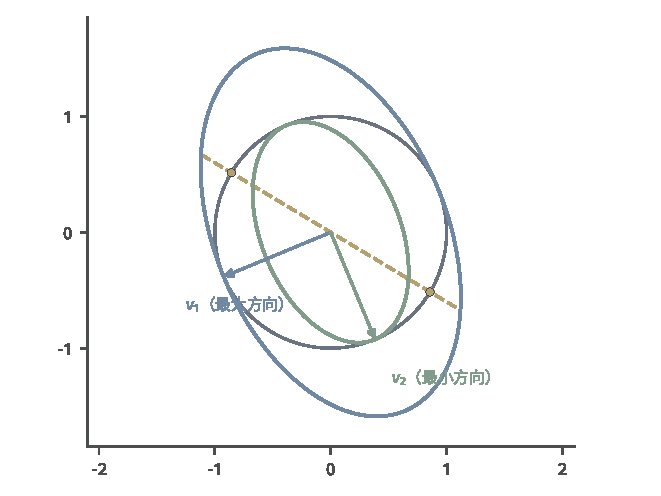
\includegraphics[width=112mm]{figures/00-shared/mathematical-preliminaries-upper/02-linear-spaces/matplotlib/ls-sphere-constrained-extremum/ls-sphere-constrained-extremum.pdf}
  \caption{单位圆约束下的极值落在特征方向。$\bm S=\left[\begin{smallmatrix}2&0.5\\0.5&1\end{smallmatrix}\right]$，
  灰圆为$\lVert\bm x\rVert=1$。蓝椭圆$\bm x^\top\bm S\bm x=\lambda_1\approx2.21$在
  $\pm\bm v_1$处与单位圆相切（最大值），绿椭圆$=\lambda_2\approx0.79$在$\pm\bm v_2$处
  相切（最小值）；黄色虚线为子空间约束直线，其上黄点是该约束下的两个极值，
  第~\ref{sec:ls-spectral-value-sensitivity}节的最小最大原理使用这种限制。
  $\lambda_{1,2}=(3\pm\sqrt2)/2$。固定复算。}
  \label{fig:ls-sphere-constrained-extremum}
\end{figure}

回到开头的对角矩阵，现在可以完成全部单位方向的比较。

\begin{example}[对角矩阵在全部单位方向上的比较]
\label{ex:ls-rayleigh-diagonal-two-by-two}
取$\bm S=\operatorname{diag}(4,1)$。每个单位向量都能写成$\bm x=(\cos\theta,\sin\theta)^\top$，其中$\theta\in[0,2\pi)$，于是
\[
 \bm x^\top\bm S\bm x=4\cos^2\theta+\sin^2\theta=1+3\cos^2\theta .
\]
由$0\leq\cos^2\theta\leq1$，它介于$1$与$4$之间：$\cos^2\theta=1$即$\bm x=\pm\bm e_1$时取最大值$4$，$\cos^2\theta=0$即$\bm x=\pm\bm e_2$时取最小值$1$。$\theta=\pi/4$时$\cos^2\theta=1/2$，得到开头的$5/2$。

可见最大值$4$与最小值$1$正是两个特征值，取到它们的方向正是特征方向，与定理~\ref{thm:matrix-analysis-rayleigh-ritz}一致；倾斜方向的值都严格介于两者之间。
\end{example}

定理不要求$\bm S$半正定。二次型可以取负值，例如$\bm S=\operatorname{diag}(1,-2)$时
\[
 \bm x^\top\bm S\bm x=x_1^2-2x_2^2 ,
\]
单位方向上的值仍介于$-2$与$1$之间，两端分别在$\pm\bm e_2$与$\pm\bm e_1$取到。

\paragraph{最优方向的唯一性}
还要区分最优值与最优方向的唯一性。最大值$\lambda_1$总是唯一的数，取到它的方向则由特征空间$\ker(\bm S-\lambda_1\bm I)$决定。

$\lambda_1$单重时，这个空间是一条直线，单位最优方向只有$\pm\bm q_1$两个，相差一个符号。$\lambda_1$重复时，空间中每个单位向量都给出最大值，例如$\bm S=\bm I$时所有单位方向都是最优的。

重根时，谱分解中的$\bm q_1$只是最优方向中的一个代表，取决于特征基的选择；最优方向组成的集合则由定理~\ref{thm:ls-spectral-projections}唯一确定。最小值的情形相同。

\paragraph{特例：$\bm S=\bm A^\top\bm A$}
一个常见的特例是$\bm S=\bm A^\top\bm A$，其中$\bm A\in\mathbb R^{m\times d}$。这时
\[
 R_{\bm A^\top\bm A}(\bm x)=\frac{\bm x^\top\bm A^\top\bm A\bm x}{\bm x^\top\bm x}=\frac{\lVert\bm A\bm x\rVert_2^2}{\lVert\bm x\rVert_2^2},
\]
即输出长度与输入长度之比的平方。

第~\ref{chap:singular-value-decomposition}章已经说明$\bm A^\top\bm A$的特征值是奇异值的平方（$d>m$时补上零）。所以定理~\ref{thm:matrix-analysis-rayleigh-ritz}给出那里最大、最小输出长度的另一种解释：单位输入的输出长度最大为$\sigma_1$，在$\bm v_1$取到；最小为$\sqrt{\lambda_d}$，其中$\lambda_d$是$\bm A^\top\bm A$的最小特征值，在它的特征方向取到。

第~\ref{sec:linear-algebra-homogeneous-estimation}节的齐次最小二乘正是在单位输入中最小化这一量。若$\bm A$有非零的零空间，最小值为零，任一单位零空间向量都最优。若$\bm A$满列秩，则$\bm A\bm x\neq\bm0$对一切$\bm x\neq\bm0$成立，$\bm A^\top\bm A\succ0$，由定理~\ref{thm:ls-symmetric-definiteness-eigenvalues}，最小值为正。

\paragraph{回到秩一逼近}
现在取$\bm S=\bm G=\bm A\bm A^\top$。由定理~\ref{thm:matrix-analysis-rayleigh-ritz}，单位方向的保留量最大为$\lambda_1(\bm G)$，恰在$\ker(\bm G-\lambda_1(\bm G)\bm I)$中的单位向量处取到。代入式~\eqref{eq:matrix-approximation-rank-one-error}，最小平方误差为
\begin{equation}
 \min_{\operatorname{rank}\bm X\leq1}\lVert\bm A-\bm X\rVert_{\mathrm F}^2=\lVert\bm A\rVert_{\mathrm F}^2-\lambda_1(\bm G) .
 \label{eq:matrix-approximation-rank-one-min-error-gram}
\end{equation}

这里只使用了第~\ref{chap:eigen-spectral-decomposition}章已经证明的谱分解。谱分解的存在不依赖本节的极值结论，本节只是用它读出极值。

\begin{example}[比较两个特征方向]
\label{ex:matrix-approximation-rank-one-eigen-directions}
沿用示例~\ref{ex:matrix-approximation-rank-one-fixed-direction}的$\bm A$。$\bm G=\bm A\bm A^\top$的元素是$\bm A$两行的内积：
\[
 g_{11}=2^2+1^2=5,\qquad g_{12}=g_{21}=2\cdot1+1\cdot2=4,\qquad g_{22}=1^2+2^2=5,
\]
即
\[
 \bm G=\begin{bmatrix}5&4\\4&5\end{bmatrix}.
\]

逐行相乘可以验证两个特征向量：
\[
 \bm G\begin{bmatrix}1\\1\end{bmatrix}=\begin{bmatrix}5+4\\4+5\end{bmatrix}=9\begin{bmatrix}1\\1\end{bmatrix},\qquad
 \bm G\begin{bmatrix}1\\-1\end{bmatrix}=\begin{bmatrix}5-4\\4-5\end{bmatrix}=\begin{bmatrix}1\\-1\end{bmatrix}.
\]
所以两个标准正交特征方向$(1,1)^\top/\sqrt2$与$(1,-1)^\top/\sqrt2$的保留量分别是$9$与$1$，重建平方误差分别是$10-9=1$与$10-1=9$。

也可以直接比较全部单位方向。取$\bm u=(\cos\theta,\sin\theta)^\top$，
\[
 \bm u^\top\bm G\bm u=5\cos^2\theta+8\cos\theta\sin\theta+5\sin^2\theta=5+4\sin2\theta ,
\]
它介于$1$与$9$之间，在$\theta=\pi/4$与$\theta=3\pi/4$分别取到最大与最小值；$\theta=0$即$\bm u=\bm e_1$时为$5$，与示例~\ref{ex:matrix-approximation-rank-one-fixed-direction}末尾的比较一致。

所以那里所取的方向$(1,1)^\top/\sqrt2$已是最优方向，而$(1,-1)^\top/\sqrt2$是最差的方向。
\end{example}

\subsection{最优解与逼近误差}
\label{sec:matrix-approximation-rank-one-solution}

\paragraph{由奇异值分解读出最优解}
上一小节用$\bm G$的特征方向给出了最优直线，现在把它与$\bm A$的奇异值分解联系起来，写出最优近似矩阵。设$\bm A\neq\bm0$，奇异值为$\sigma_1\geq\cdots\geq\sigma_r>0$。

式~\eqref{eq:ls-svd-transpose-relation}说明，$\bm G=\bm A\bm A^\top$的特征值是$\sigma_1^2,\ldots,\sigma_r^2$及$m-r$个零，左奇异向量$\bm u_i$是对应的特征向量。因此最大保留量为$\lambda_1(\bm G)=\sigma_1^2$，取$\bm u=\bm u_1$即可达到。

总平方长度也由奇异值给出：
\[
 \lVert\bm A\rVert_{\mathrm F}^2=\operatorname{tr}\bm G=\sum_{i=1}^r\sigma_i^2 .
\]
所以最小平方误差为
\begin{equation}
 \lVert\bm A\rVert_{\mathrm F}^2-\sigma_1^2=\sum_{i=2}^r\sigma_i^2 .
 \label{eq:matrix-approximation-rank-one-min-error}
\end{equation}

再求最优系数。由式~\eqref{eq:ls-svd-transpose-relation}，$\bm A^\top\bm u_1=\sigma_1\bm v_1$，所以
\[
 \bm c=\bm A^\top\bm u_1=\sigma_1\bm v_1 .
\]
把最佳方向与最优系数合成：
\begin{equation}
 \bm A_1=\bm u_1\bm u_1^\top\bm A=\bm u_1(\bm A^\top\bm u_1)^\top=\sigma_1\bm u_1\bm v_1^\top .
 \label{eq:matrix-approximation-rank-one-optimum}
\end{equation}

这是原矩阵$\bm A$的秩一近似，即和式~\eqref{eq:matrix-analysis-svd-rank-one-sum}的第一项，而不是Gram矩阵$\bm G$的秩一近似。计算的输入是$\bm A$，输出是近似矩阵$\bm A_1$；它不是某个方程的解向量。

\paragraph{计算步骤}
按上面的推导，计算秩一最优逼近只需三件事：求出保留量最大的方向，求出各列在该方向上的系数，再把两者合成。下面写出用到的变量与步骤，并用以下数据逐步演示：
\[
 \bm A=\begin{bmatrix}2&1\\1&2\end{bmatrix}.
\]
这是示例~\ref{ex:matrix-approximation-rank-one-fixed-direction}的矩阵。

变量如下。
\begin{itemize}
 \item $\sigma_1^2$与$\bm u_1\in\mathbb R^m$：$\bm G=\bm A\bm A^\top$的最大特征值与一个单位特征向量，即最大保留量与最优方向。
 \item $\bm c\in\mathbb R^d$：各列在$\bm u_1$上的投影系数，等于$\sigma_1\bm v_1$。
 \item $\bm A_1\in\mathbb R^{m\times d}$：秩一近似矩阵。
 \item $e$：平方误差$\lVert\bm A-\bm A_1\rVert_{\mathrm F}^2$，用于核对。
\end{itemize}

依次执行以下步骤。
\begin{enumerate}
 \item \textbf{求最优方向。}求$\bm G=\bm A\bm A^\top$的最大特征值$\sigma_1^2$与单位特征向量$\bm u_1$；若已有$\bm A$的奇异值分解，直接读出$\sigma_1$与$\bm u_1$。例中示例~\ref{ex:matrix-approximation-rank-one-eigen-directions}已求得
 \[
  \sigma_1^2=9,\qquad \bm u_1=\frac1{\sqrt2}\begin{bmatrix}1\\1\end{bmatrix}.
 \]

 \item \textbf{求系数。}按式~\eqref{eq:matrix-approximation-rank-one-coefficients}计算
 \[
  \bm c=\bm A^\top\bm u_1 .
 \]
 例中
 \[
  \bm c=\frac1{\sqrt2}\begin{bmatrix}2+1\\1+2\end{bmatrix}=\frac3{\sqrt2}\begin{bmatrix}1\\1\end{bmatrix}.
 \]
 它等于$\sigma_1\bm v_1$，其中$\sigma_1=3$、$\bm v_1=(1,1)^\top/\sqrt2$；已有奇异值分解时这一步可直接取$\sigma_1\bm v_1$。

 \item \textbf{合成近似矩阵。}按式~\eqref{eq:matrix-approximation-rank-one-optimum}作外积
 \[
  \bm A_1=\bm u_1\bm c^\top .
 \]
 例中
 \[
  \bm A_1=\frac1{\sqrt2}\cdot\frac3{\sqrt2}\begin{bmatrix}1&1\\1&1\end{bmatrix}=\frac32\begin{bmatrix}1&1\\1&1\end{bmatrix}.
 \]

 \item \textbf{核对误差。}求残差$\bm A-\bm A_1$的平方和，并与$\lVert\bm A\rVert_{\mathrm F}^2-\sigma_1^2$比较。例中
 \[
  \bm A-\bm A_1=\frac12\begin{bmatrix}1&-1\\-1&1\end{bmatrix},\qquad
  e=1=10-9 .
 \]
\end{enumerate}

最终得到
\[
 \bm A_1=\frac32\begin{bmatrix}1&1\\1&1\end{bmatrix}.
\]
它的四个元素都是$3/2$，两列成比例，秩为一。另一个奇异值是$\sigma_2=1$（$\bm A(1,-1)^\top=(1,-1)^\top$），平方误差$1=\sigma_2^2$，与最小误差公式一致。

同样的步骤用于示例~\ref{ex:ls-low-rank-three-columns}。这时$\bm G=\operatorname{diag}(9,4,1)$，最大特征值为$9$，$\bm u_1=\bm e_1$。系数与合成的近似矩阵为
\[
 \bm c=\bm A^\top\bm e_1=\begin{bmatrix}3\\0\\0\end{bmatrix},\qquad \bm A_1=3\bm e_1\bm e_1^\top .
\]
它只保留第一列，另两列被投影成零，平方误差为
\[
 14-9=5=4+1 .
\]

\paragraph{列重建与行重建}
这里用的是$\bm A\bm A^\top$而不是$\bm A^\top\bm A$，因为我们重建的是$\mathbb R^m$中的列向量。保留量直接等于列向量在$\bm u$上的投影长度平方之和，对应的是左奇异方向。

若改为重建行向量，同样的推导会用到$\bm A^\top\bm A$与右奇异方向$\bm v_1$。由$\bm A\bm v_1=\sigma_1\bm u_1$，得到的近似是
\[
 \bm A\bm v_1\bm v_1^\top=\sigma_1\bm u_1\bm v_1^\top ,
\]
与式~\eqref{eq:matrix-approximation-rank-one-optimum}是同一个矩阵。

这种解释依赖$\bm G$是Gram矩阵。对一般不定的对称矩阵$\bm S$，二次型值可能为负，不能把任意Rayleigh商的极值都解释成某个矩阵的最佳秩一逼近。

\paragraph{最优矩阵的唯一性}
最后区分最优近似矩阵与它的表示。$\bm A=\bm0$时$r=0$，每个方向的保留量都是零，唯一的最优近似是零矩阵。

$\sigma_1>\sigma_2$（或$r=1$）时，$\bm G$最大特征值的特征空间是一条直线，最优方向只有$\pm\bm u_1$。把$(\bm u_1,\bm v_1)$同时换成$(-\bm u_1,-\bm v_1)$不改变外积，所以最优矩阵$\bm A_1$唯一，不唯一的只是它的写法。

$\sigma_1=\sigma_2$时情况不同：最大特征值的特征空间至少二维，其中每个单位向量$\bm u$都给出最优近似$\bm u\bm u^\top\bm A$，不同的直线给出不同的矩阵。例如$\bm A=\bm I_2$时，$\bm G=\bm I_2$，每个单位向量$\bm u$的保留量都是$1$，误差都是
\[
 \lVert\bm I_2-\bm u\bm u^\top\rVert_{\mathrm F}^2=2-1=1 ;
\]
$\bm e_1\bm e_1^\top$与$\bm e_2\bm e_2^\top$就是两个不同的最优近似。

所以表示的非唯一性不等于近似矩阵的非唯一性，后者只来自最大奇异值重复。下一步保持误差标准不变，把允许保留的方向数由一个增加到$k$个。
